\documentclass[12pt, a4paper]{article}
% Immagini
\usepackage{graphicx}
% Formule matematiche
\usepackage{amsmath}
% Margini e Impaginazione
\usepackage{geometry}
\usepackage{amsmath}
\usepackage{amsfonts}
% Link
\usepackage{hyperref}
% Load the parskip package with skip and indent options
\usepackage{parskip}
% Tables
\usepackage[normalem]{ulem}
\useunder{\uline}{\ul}{}
% Code
\usepackage{listings}
\usepackage{color}

\usepackage[caption=false]{subfig}

\definecolor{dkgreen}{rgb}{0,0.6,0}
\definecolor{gray}{rgb}{0.5,0.5,0.5}
\definecolor{mauve}{rgb}{0.58,0,0.82}

\lstset{frame=tb,
  language=Java,
  aboveskip=3mm,
  belowskip=3mm,
  showstringspaces=false,
  columns=flexible,
  basicstyle={\small\ttfamily},
  numbers=none,
  numberstyle=\tiny\color{gray},
  keywordstyle=\color{blue},
  commentstyle=\color{dkgreen},
  stringstyle=\color{mauve},
  breaklines=true,
  breakatwhitespace=true,
  tabsize=3
}

\hypersetup{
  colorlinks=true,
  linkcolor=blue,
  filecolor=magenta,      
  urlcolor=blue,
}
\geometry{a4paper, top=3cm, bottom=3cm, left=2.5cm, right=2.5cm, heightrounded, bindingoffset=5mm}


\begin{document}
\author{Carlo Marra}
\title{Sviluppo di un'applicazione software per la generazione automatica di playlist attraverso la ricerca ricorsiva e grafi pesati}
\date{Anno accademico 2023/2024}
\begin{figure}[h]
  \centering
  
\includegraphics[width=0.7\linewidth]{images/polito_logo_2021_blu}
\end{figure}

\begin{center}
  \LARGE{\textbf{Politecnico di Torino}}
\end{center}
\begin{center}
  \Large{Corso di Laurea in Ingegneria Gestionale\\A.a. 2023/2024}
\end{center}

\begin{center}
  \LARGE{Sviluppo di un'applicazione software\\ per la generazione automatica di playlist\\ attraverso la ricerca ricorsiva e grafi pesati}
\end{center}
\section*{ }
Relatore: Fulvio Corno\\
Candidato: Carlo Marra

\thispagestyle{empty} 
\newpage

\tableofcontents
\thispagestyle{empty} 
\newpage
\setcounter{page}{1}
\section{Problema proposto}

\subsection{Studente proponente}
s249863 \\ Carlo Marra 

\subsection{Titolo della proposta}

Sviluppo di un'applicazione software per la generazione automatica di playlist attraverso la ricerca ricorsiva e grafi pesati.

\subsection{Descrizione del problema proposto}

Creare una playlist soddisfacente è una sfida comune per ogni individuo. Ogni persona ha gusti musicali unici e mutevoli, rendendo difficile la selezione di brani che rispecchino perfettamente il proprio umore e le preferenze del momento.\par La vasta gamma di generi musicali, artisti e canzoni disponibili rende ancora più complicata la creazione di una playlist che riesca a catturare l'essenza di chi siamo. La soluzione proposta mira alla ricerca della miglior playlist possibile a seguito di alcune linee guida dell’utente.

\subsection{Descrizione della rilevanza gestionale del problema}
Per molti individui, trovare una playlist adatta alla situazione può svolgere un ruolo significativo nella motivazione per iniziare un progetto o un viaggio. La musica ha il potere di influenzare le nostre emozioni, creando l'atmosfera e l'energia desiderate. Una playlist ben selezionata può stimolare la creatività, migliorare il focus, la produttività e amplificare l'entusiasmo per l'attività imminente.

\subsection{Descrizione dei data-set per la valutazione}
Il data-set utilizzato sarà ispirato a “Spotify - All Time Top 2000s Mega Dataset“. Questo dataset contiene le statistiche audio di 2000 brani tra i più ascoltati su Spotify. Sono inclusi brani pubblicati dal 1956 al 2019 di artisti noti e famosi come Queen, The Beatles, Guns N' Roses, ecc. \par Questi dati sono estratti dalla playlist di Spotify “Top 2000s“\footnote{http://sortyourmusic.playlistmachinery.com} utilizzando Selenium con Python.
\newpage

\subsection{Descrizione preliminare degli algoritmi coinvolti}
L'applicazione si dividerà in due sezioni indipendenti: la sezione "Surprise Me" e la sezione "My Mix".

\textbf{Sezione "Surprise Me"}

L’utente avrà il compito di specificare alcuni requisiti che il risultato dovrà soddisfare. Tra queste vi sono:
\begin{itemize}
\item Il genere musicale della playlist desiderata e, una volta scelto, facoltativamente l’artista preferito appartenente al genere scelto precedentemente.
\item Il grado di presenza richiesta delle cinque caratteristiche principali, Energia (E), Ballabilità (D), Positività (V), Acustica (A) e Popolarità (P) attraverso un punteggio da 1 a 10.
\end{itemize}

Gli input ricevuti saranno usati per creare un grafo pesato in cui i nodi saranno tutte le canzoni che soddisfano il genere scelto.
Ad ogni traccia verrà attribuito un punteggio di affinità con le cinque caratteristiche richieste.
Dati i cinque gradi ($G_i$) ricevuti e ciascun brano $B_i$ che rientra nel genere scelto:
$$ \text{Punteggio}(B_i) = G_E \cdot E(B_i) + G_D \cdot D(B_i) + G_V \cdot V(B_i) + G_A \cdot A(B_i) + G_P \cdot P(B_i) $$
Attraverso questo punteggio associato a ciascun vertice, il peso di ciascun arco sarà calcolato attraverso la differenza (in valore assoluto) di punteggio dei due nodi considerati, di conseguenza un peso basso corrisponderà ad un alta affinità. \par
Una volta ottenuto il grafo, si procederà con una ricerca ricorsiva (opportunamente ottimizzata) che troverà la playlist con il più basso valore totale di archi percorsi. In caso di più possibili affinità con il brano successivo e la presenza di una brano dell’artista preferito, la scelta ricadrà su quest’ultimo in caso di pesi degli archi simili. \par
L’idea di limitare la ricerca ad un singolo genere potrà essere allargata a due o più in caso di buone prestazioni dell’algoritmo.
La playlist trovata sarà poi inserita all’interno della tabella dell’applicazione software e il suo punteggio all’intento della casella di testo sottostante.

\newpage
\textbf{Sezione "My Mix"}

L'utente potrà aggiungere, prima della ricerca, le sue canzoni preferite inserendo rispettivamente genere, artista e brano.
Una volta aggiunte, potrà decidere il numero massimo di canzoni nella playlist o il numero massimo di minuti totali.
A quel punto si procederà allo studio delle canzoni inserite per creare una playlist che sia coerente per genere e attributi. \par
Per la determinazione dei gusti dell'utente si farà la media della somma di ciascun attributo del brano i-esimo ($B_i$).
Preso come esempio l'attributo "Popolarità" e $N$ brani in input:
$$ \bar P = \frac{\sum_{i=1}^NP(i)}{N} $$
Il punteggio di ciascun potenziale brano sarà quindi:
$$ \text{Punteggio}(B_i) = \frac{\bar E}{10} \cdot E(B_i) + \frac{\bar D}{10} \cdot D(B_i) + \frac{\bar V}{10} \cdot V(B_i) + \frac{\bar A}{10} \cdot A(B_i) + \frac{\bar P}{10} \cdot P(B_i) $$
La divisione di ciascun fattore per 10 è solamente per rendere i punteggi consistenti con quelli della prima sezione (da $1$ a $10$).\par
Si procederà quindi, come nella sezione precedente, alla creazione del grafo pesato con le relative affinità e alla ricerca ricorsiva della playlist ottima.


\subsection[Descrizione preliminare delle funzionalità previste per l’applicazione software]{Descrizione preliminare delle funzionalità\\*previste per l’applicazione software}

L’applicazione software di ciascuna delle due sezioni sarà divisa graficamente in due VBox, una a sinistra e una a destra, rispettivamente per la descrizione delle preferenze e per la visione del risultato ottenuto. In ciascuna Tab si avrà nella parte bassa una Label che conterrà alcune linee guida per la buona riuscita dell’applicazione e una piccola descrizione di ciascun valore degli Slider.

\textbf{Sezione "Surprise Me"}

La parte di sinistra della sezione "Surprise Me" conterrà:
\begin{itemize}
\item Due TextArea per la scelta del numero massimo di brani richiesto e per i minuti massimi totali della playlist. Queste due TextArea saranno accompagnate da due CheckBox per segnalare quali dei due vincoli l’utente preferisce che venga rispettato.
\item Una ChoiceBox per la scelta del genere preferito e una ChoiceBox per la scelta dell’artista preferito. Questa verrà compilata al momento della scelta del genere preferito.
\item Cinque Slider orizzontali che, attraverso una scala da 1 a 10, serviranno all’utente per condividere i propri gusti e aspettative sulla playlist finale. I cinque attributi degli Slider saranno Energia, Ballabilità, Positività, Acustica e Popolarità.
\item Due bottoni per il reset degli input e per l’avvio della ricerca.
\end{itemize}
\newpage
La VBox di destra conterrà:
\begin{itemize}
\item Una tabella per la visualizzazione del risultato finale.
\item Una casella di testo non modificabile per alcune statistiche legate al risultato finale.
\end{itemize}

\textbf{Sezione "My Mix"}

La parte di sinistra conterrà nello specifico:
\begin{itemize}
\item Due TextArea per la scelta del numero massimo di brani richiesto e per i minuti massimi totali della playlist. Queste due TextArea saranno accompagnate da due CheckBox per segnalare quali dei due vincoli l’utente preferisce che venga rispettato.
\item Una ChoiceBox per la scelta del genere preferito. Il genere scelto servirà a costruire il grafo su cui eseguire la ricerca.
\item Una ChoiceBox per la scelta dell’artista preferito. Questa verrà compilata al momento della scelta del genere preferito.
\item Una ChoiceBox per la scelta del brano dell'artista preferito. Questa verrà compilata al momento della scelta dell'artista preferito.
\item Quattro Buttons, rispettivamente per il reset degli input, per l'aggiunta della canzone selezionata alla playlist di partenza, per l'eliminazione dell'ultimo brano inserito e per l'avio della ricerca.
\end{itemize}

La VBox di destra conterrà:
\begin{itemize}
\item Una tabella per la visualizzazione del risultato finale.
\item Una casella di testo non modificabile per alcune statistiche legate al risultato finale.
\end{itemize}

\newpage
\section{Descrizione del problema affrontato}

\subsection{Contesto operativo}

Mettendosi nei panni di un'azienda che opera nel campo del mercato  musicale, risulta evidente come la possibilità di consigliare playlist personalizzate ai propri utenti offre diversi vantaggi sia per gli utenti che per l'azienda stessa. Tra questi è possibile trovare:
\begin{itemize}
\item \textbf{Fidelizzazione degli utenti}: Offrire playlist personalizzate crea un'esperienza più coinvolgente per gli utenti, che si sentono compresi e apprezzati.
\item \textbf{Aumento dell'engagement}: Le playlist personalizzate tengono gli utenti impegnati sulla piattaforma musicale più a lungo, aumentando il tempo complessivo trascorso e il coinvolgimento complessivo degli utenti.
\item \textbf{Opportunità di cross-selling}: Attraverso la conoscenza dei gusti musicali degli utenti, un'azienda musicale può anche suggerire altri servizi o prodotti correlati che potrebbero interessare, creando opportunità di vendita incrociata.
\item \textbf{Raccolta di dati utili}: L'analisi dei dati generati dalle preferenze musicali degli utenti fornisce informazioni preziose sull'andamento del mercato, i trend emergenti e le preferenze della clientela. Questi dati possono essere sfruttati per migliorare ulteriormente i servizi offerti e adeguare l'offerta alle esigenze degli utenti.
\end{itemize}

\subsection{Descrizione del sotto-problema}

Come accennato nel punto dell'\textbf{Aumento dell'engagement} del sotto-paragrafo precedente, un algoritmo per la creazione di playlist musicali basato su input numerici o preferenze personali offre una serie di vantaggi pratici e emotivi, migliorando l'accesso alla musica e arricchendo l'esperienza degli utenti nel loro contesto quotidiano. L'utente finale trarrà diversi vantaggi nell'impiego di questo algoritmo, tra cui:
\begin{itemize}
\item \textbf{Supporto emotivo e motivazionale}: La capacità di considerare parametri come il grado di positività o energia può essere utilizzata per creare playlist che si adattano alle diverse esigenze emotive degli utenti. Ad esempio, una playlist di alta energia potrebbe essere adatta per un allenamento fisico, mentre una playlist più rilassante potrebbe essere preferita per il relax serale.
\item \textbf{Risparmio di tempo}: Nel contesto di playlist generate automaticamente, un algoritmo può risparmiare tempo agli utenti nell'individuare manualmente brani adatti ai loro stati d'animo o attività. L'automazione del processo di selezione della musica consente alle persone di concentrarsi su altre attività senza dover creare manualmente playlist o cercare singoli brani.
\item \textbf{Contesto sociale e condivisione}: Algoritmi di questo tipo possono anche facilitare la condivisione e la scoperta di nuovi brani tra gli utenti con gusti simili. La capacità di suggerire canzoni in base a preferenze simili può favorire una maggiore connessione sociale attraverso la condivisione di esperienze musicali.
\end{itemize}

\newpage
\section{Dataset utilizzato}

\subsection{Introduzione}

Il dataset utilizzato è basato su “Spotify - All Time Top 2000s Mega Dataset“\footnote{https://www.kaggle.com/datasets/iamsumat/spotify-top-2000s-mega-dataset}. Quest'ultimo contiene le statistiche audio di 2000 brani tra i più ascoltati su Spotify. I dati sono estratti dalla playlist di Spotify “Top 2000s“ su PlaylistMachinery\footnote{http://sortyourmusic.playlistmachinery.com} utilizzando Selenium con Python.\par
Al fine di ottenere risultati consistenti per ogni tipo di playlist richiesta, il dataset di partenza è stato alterato mediante l'aggregazione di tracce di sottogeneri poco frequenti all'interno di un genere principale, con l'obiettivo di assicurare almeno 20 brani associati per ciascun genere.

\subsection{Tabella \textit{tracks}}

\begin{table}[h]
\centering
\begin{tabular}{ll|}
\hline
\multicolumn{2}{|c|}{\textit{\textbf{tracks}}} \\ \hline
\multicolumn{1}{|l|}{{\ul PK}} & Index \\ \hline
\multicolumn{1}{l|}{} & Title \\ \cline{2-2} 
\multicolumn{1}{l|}{} & Artist \\ \cline{2-2} 
\multicolumn{1}{l|}{} & Top Genre \\ \cline{2-2} 
\multicolumn{1}{l|}{} & Year \\ \cline{2-2} 
\multicolumn{1}{l|}{} & Beats per Minute (BPM) \\ \cline{2-2} 
\multicolumn{1}{l|}{} & Length \\ \cline{2-2} 
\multicolumn{1}{l|}{} & Loudness (DB) \\ \cline{2-2} 
\multicolumn{1}{l|}{} & Energy \\ \cline{2-2} 
\multicolumn{1}{l|}{} & Danceability \\ \cline{2-2} 
\multicolumn{1}{l|}{} & Acoustic \\ \cline{2-2} 
\multicolumn{1}{l|}{} & Speechiness \\ \cline{2-2} 
\multicolumn{1}{l|}{} & Popularity \\ \cline{2-2} 
\end{tabular}
\end{table}

La tabella utilizzata per la creazione del software è composta dai seguenti attributi:
\begin{itemize}
\item Index: Identificativo della traccia e PK della tabella;
\item Title: Nome della traccia;
\item Artist: Nome dell'artista;
\item Top Genre: Genere della traccia;
\item Year: Anno di pubblicazione della traccia;
\item Beats per Minute (BPM): Il tempo della canzone in battiti per minuto;
\item Length: La durata della canzone in secondi;
\item Loudness (dB): Maggiore è il valore, più alta è la canzone;
\end{itemize}
I seguenti attributi, descrittivi delle caratteristiche principali di ciascun brano, sono espressi in valori interi compresi tra 0 e 100:
\begin{itemize}
\item Energy: L'energia di una canzone - maggiore è il valore, più energica è la canzone;
\item Danceability: Maggiore è il valore, più facile è ballare su questa canzone;
\item Valence: Maggiore è il valore, più positivo è l'umore della canzone;
\item Acoustic: Maggiore è il valore, più acustica è la canzone;
\item Speechiness: Maggiore è il valore, più parole parlate contiene la canzone;
\item Popularity: Maggiore è il valore, più popolare è la canzone.
\end{itemize}

\newpage
\section{View (scene.fxml)}

La View è responsabile della presentazione dei dati e dell'interazione con l'utente, assicurando che l'interfaccia utente sia intuitiva, risponda dinamicamente ai cambiamenti nel Model e fornisca un feedback chiaro durante l'utilizzo dell'applicazione.

Le interfacce grafiche sono state realizzate in \textit{JavaFX}, utilizzando l’applicativo \newline \textit{SceneBuilder}. 

La scena ideata è divisa in due Tab denominati rispettivamente "Surprise Me" e "My Mix".

\subsection{Elementi comuni}
Nel lato in alto a sinistra di entrambi i Tab è presente la possibilità di selezionare uno dei due vincoli che la playlist dovrà rispettare, cioè il numero di minuti totali dei brani al suo interno o più semplicemente il numero totale di brani. 

I due vincoli sono stati implementati con due RadioButton affiancati da una ComboBox per selezionare il numero di brani desiderato (valori che vanno da 10 fino ad un massimo di 30) e da un TextField in cui specificare la somma di minuti totali. I valori accettati di quest'ultimo sono stati limitati a 180 minuti.

\begin{figure}[h]
  \centering
  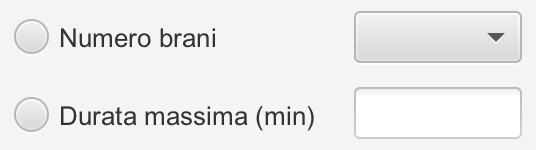
\includegraphics[width=0.5\linewidth]{images/vincolo_comune.png}
  \caption{Vincoli comuni}
\end{figure}

Le due Tab condividono un TableView con due colonne, "Artista" e "Titolo", in cui sarà inserita la playlist ottima al termine della ricerca. 
Al di sotto della TableView vi è una TextArea non modificabile dall'utente dove sarà possibile ispezionare il numero di brani della playlist e il numero di minuti totali.

Un'altra caratteristica presente in entrambi i Tab è una Label nella parte bassa della window in cui sono presenti le istruzioni per poter utilizzare al meglio l'applicazione.

\subsection{Surprise Me}
La sezione "Surprise Me" è composta da una SplitPane in cui nella zona a sinistra sono presenti i controlli dedicati all'utente per la specificazione delle proprie preferenze e nella zona di destra una tabella in cui verrà visualizzata la playlist in output.

Al di sotto dei vincoli in comune (v. Elementi comuni) vi è la possibilità di scegliere il proprio genere preferito e, facoltativamente, l'artista preferito associato attraverso due ComboBox.

\begin{figure}[h]
  \centering
  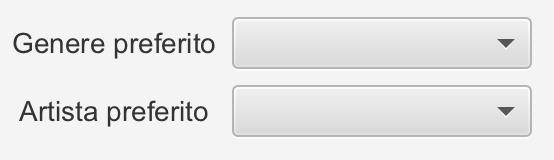
\includegraphics[width=0.5\linewidth]{images/surpriseme_genre_artist.png}
  \caption{ComboBox per la scelta del genere e dell'artista preferito}
\end{figure}

\newpage
Sono presenti infine cinque Slider per indicare rispettivamente il grado di presenza richiesta delle cinque caratteristiche principali associate a ciascun brano, Energy (E), Danceability (D), Valence (V), Acoustic (A) e Popularity (P) attraverso un punteggio da 1 a 10. 

\begin{figure}[h]
  \centering
  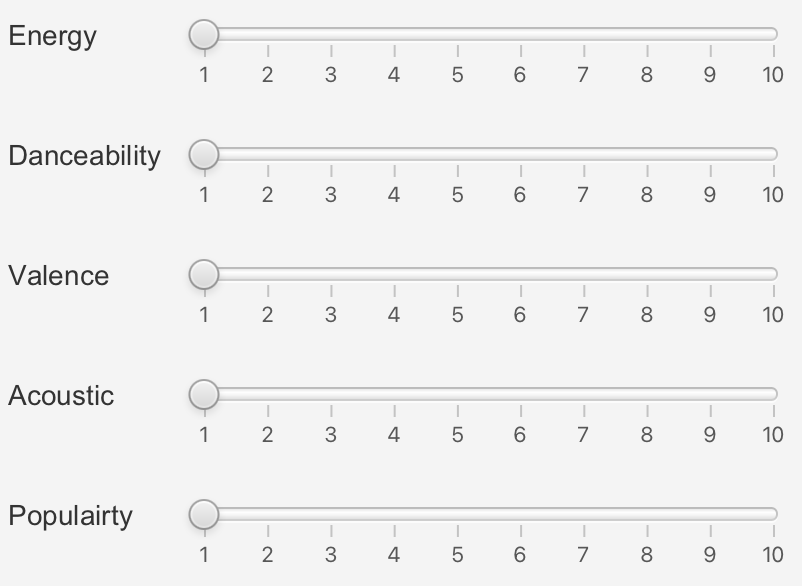
\includegraphics[width=0.8\linewidth]{images/sliders.png}
  \caption{Sliders}
\end{figure}

I cinque slider sono seguiti da due Button, uno per il reset dei valori fino a quel momento specificati e l'altro per l'avvio della ricerca della miglior playlist.

\begin{figure}[h]
  \centering
  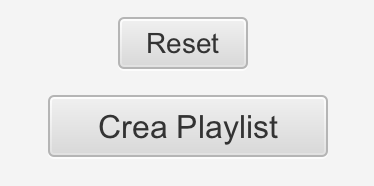
\includegraphics[width=0.3\linewidth]{images/surpriseme_buttons.png}
  \caption{Buttons per reset e avvio della ricerca}
\end{figure}

\newpage 
\subsection{My Mix}

La sezione "My Mix" è composta da una SplitPane la cui zona a sinistra permette all'utente l'inserimento dei brani preferiti su cui verrà effettuato lo studio dei gusti e la conseguente ricerca. Nella zona di destra, come nella sezione precedente, è presente una tabella in cui verrà visualizzata la playlist in output.

L'inserimento all'interno della playlist dei brani preferiti avviene attraverso la selezione in fila del genere, artista e infine del brano desiderato attraverso tre ComboBox che si riempiono conseguentemente alle precendenti scelte effettutate.

 \begin{figure}[h]
  \centering
  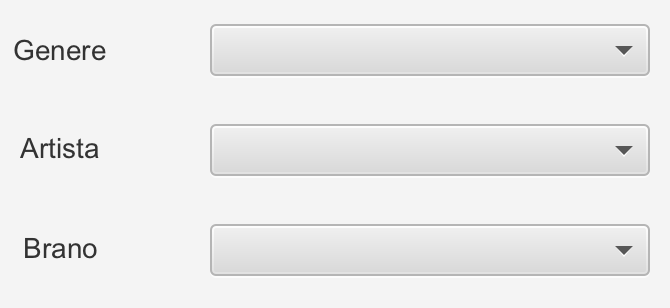
\includegraphics[width=0.6\linewidth]{images/mymix_combobox.png}
  \caption{ComboBox per la selezione del brano da inserire nella TableView}
\end{figure}

Le precedenti ComboBox sono seguite da quattro Buttons:
\begin{itemize}
\item Aggiungi: Aggiungere il brano selezionato alla TableView;
\item Reset: Inizializzazione delle scelte effettuate all'interno delle ComboBox;
\item Inizializza Playlist: rimozione di tutti i brani fino a quel momento aggiunti alla TableView;
\item Rimuovi ultimo brano: rimozione dell'ultimo brano aggiunto alla TableView.
\end{itemize}

 \begin{figure}[h]
  \centering
  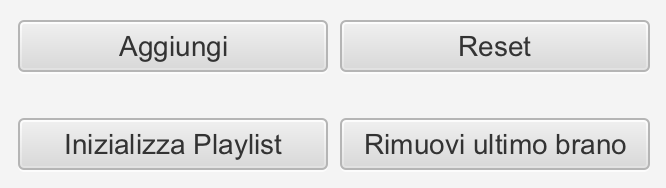
\includegraphics[width=0.6\linewidth]{images/mymix_buttons.png}
  \caption{Buttons della sezione "My Mix"}
\end{figure}

La splitPane di sinistra è infine conclusa con un Button per l'avvio della ricerca della playlist ottima.

\newpage

\begin{figure}[ht]
\centering
  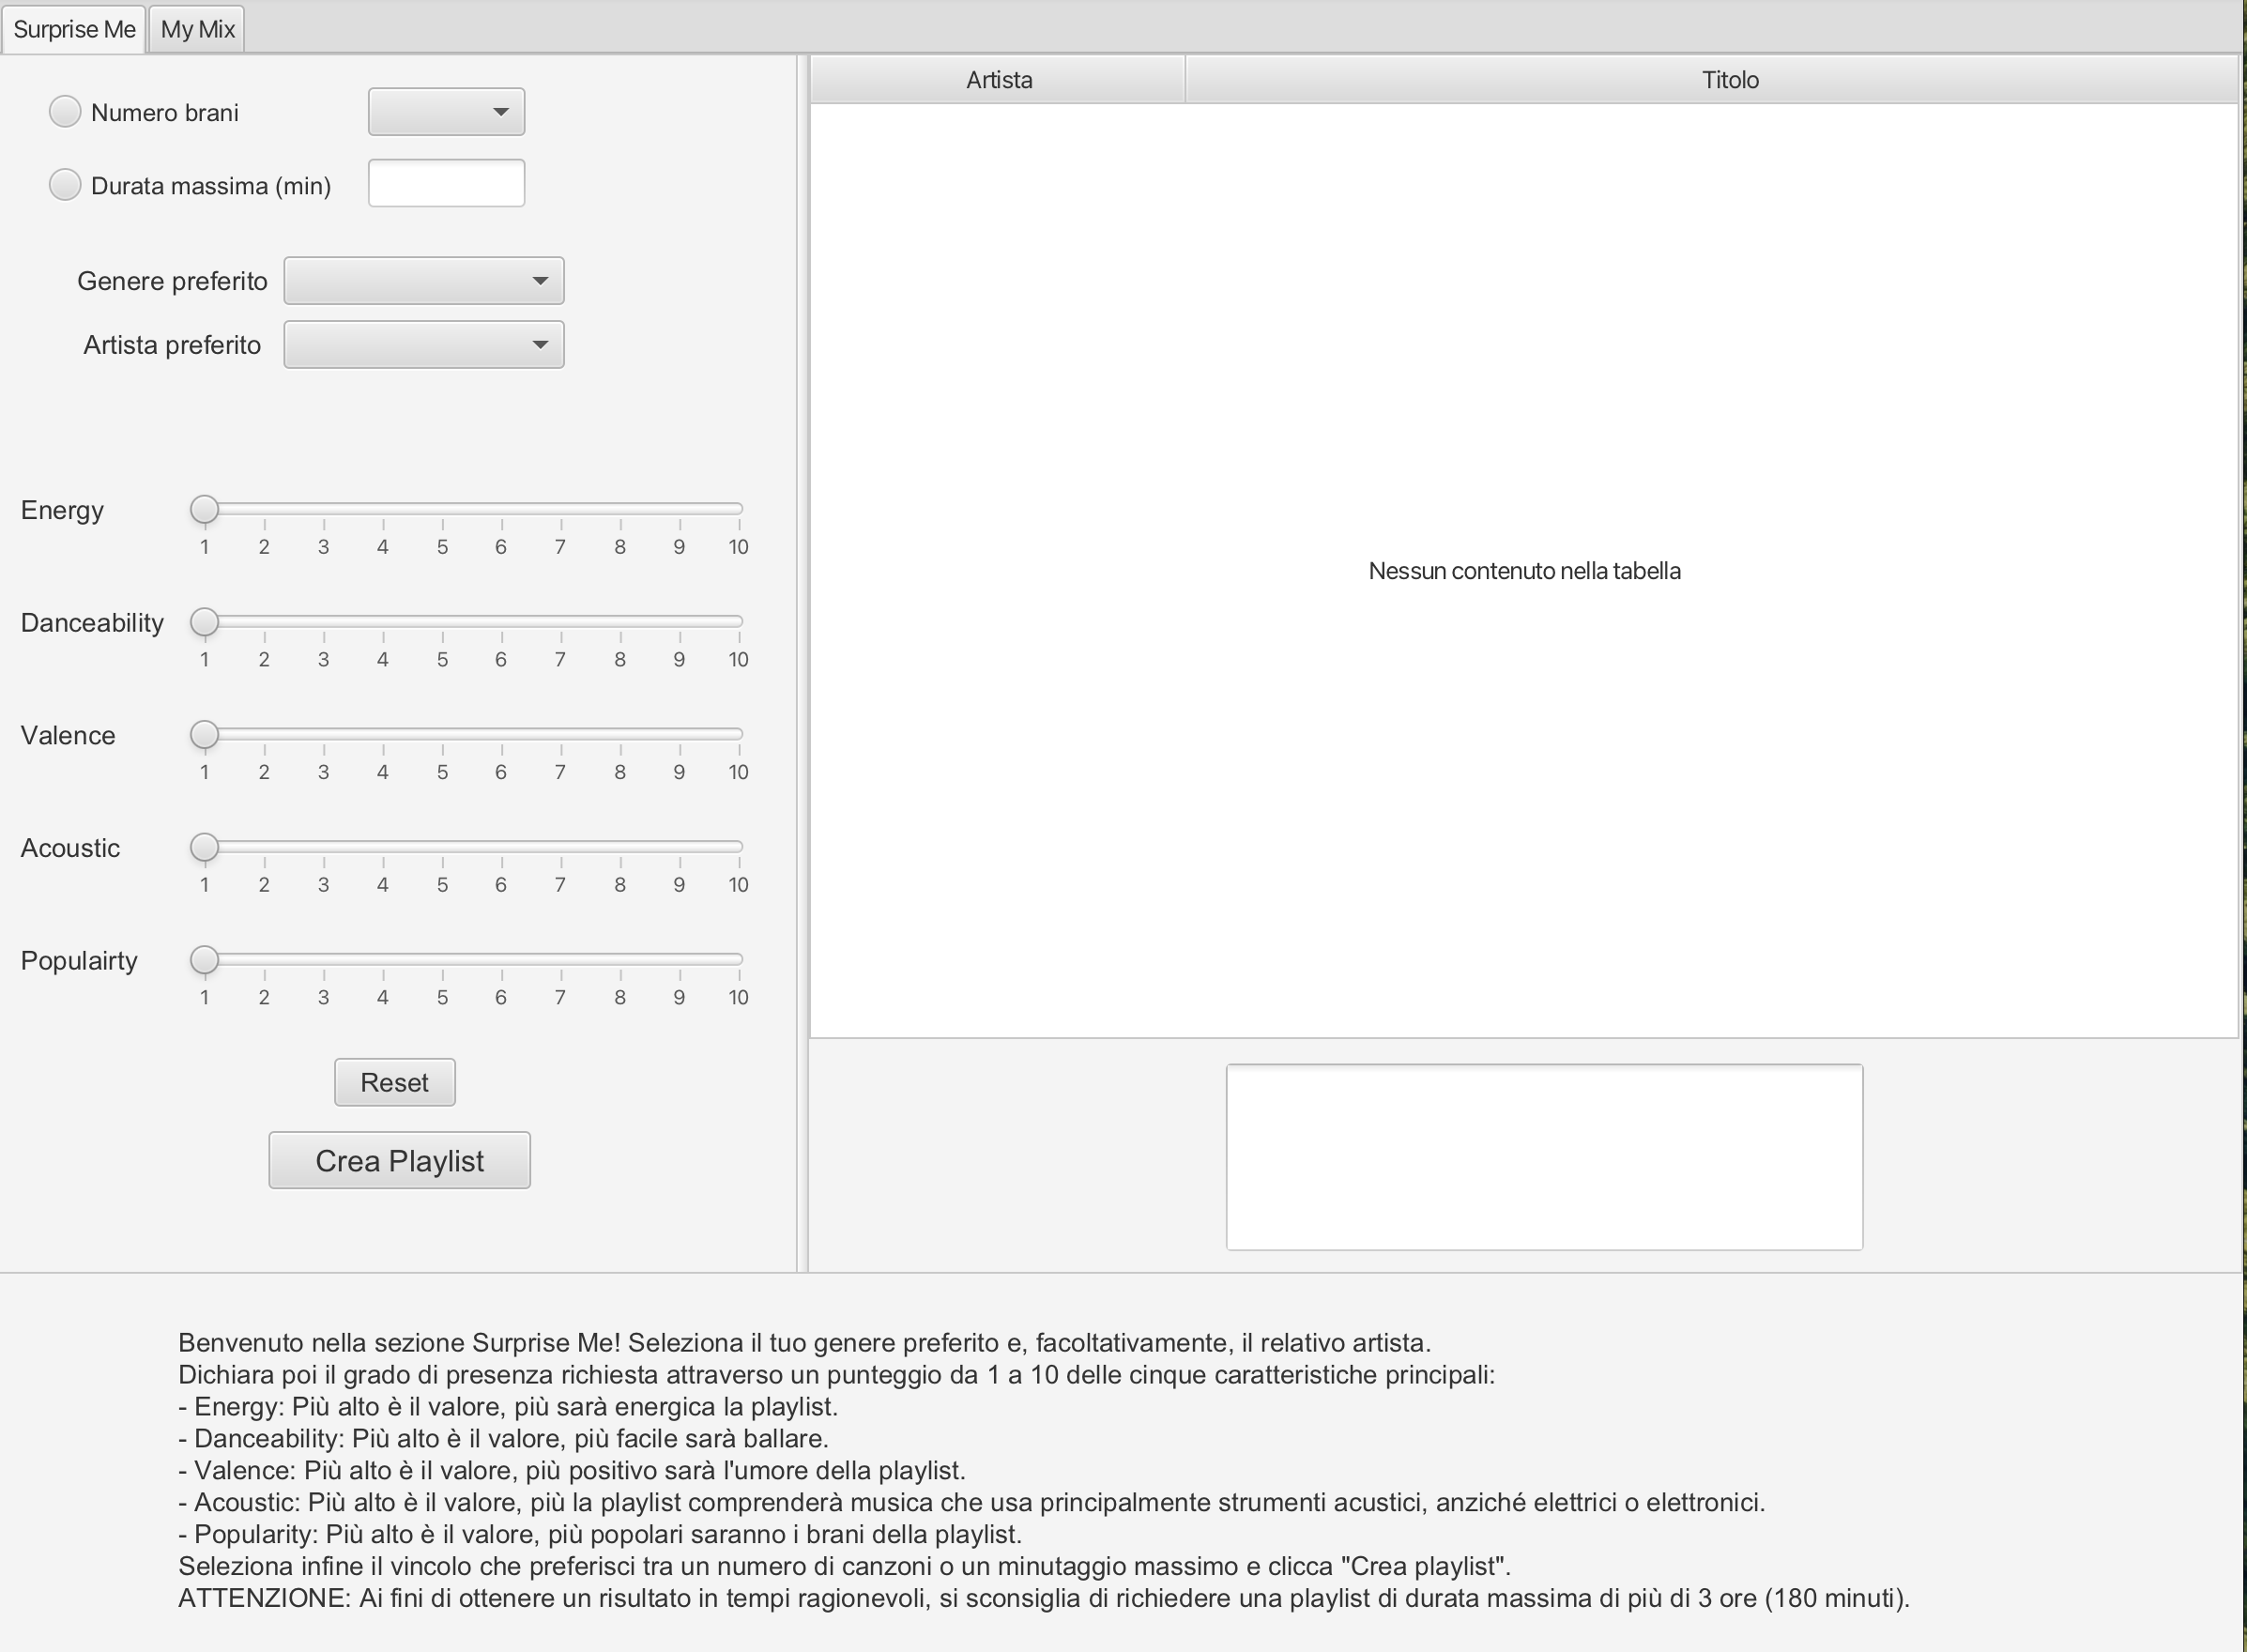
\includegraphics[clip, width=0.65\linewidth]{images/surpriseMeTotal.png}
  \caption{Surprise Me tab}
\end{figure}
  
\begin{figure}[ht]  
\centering
  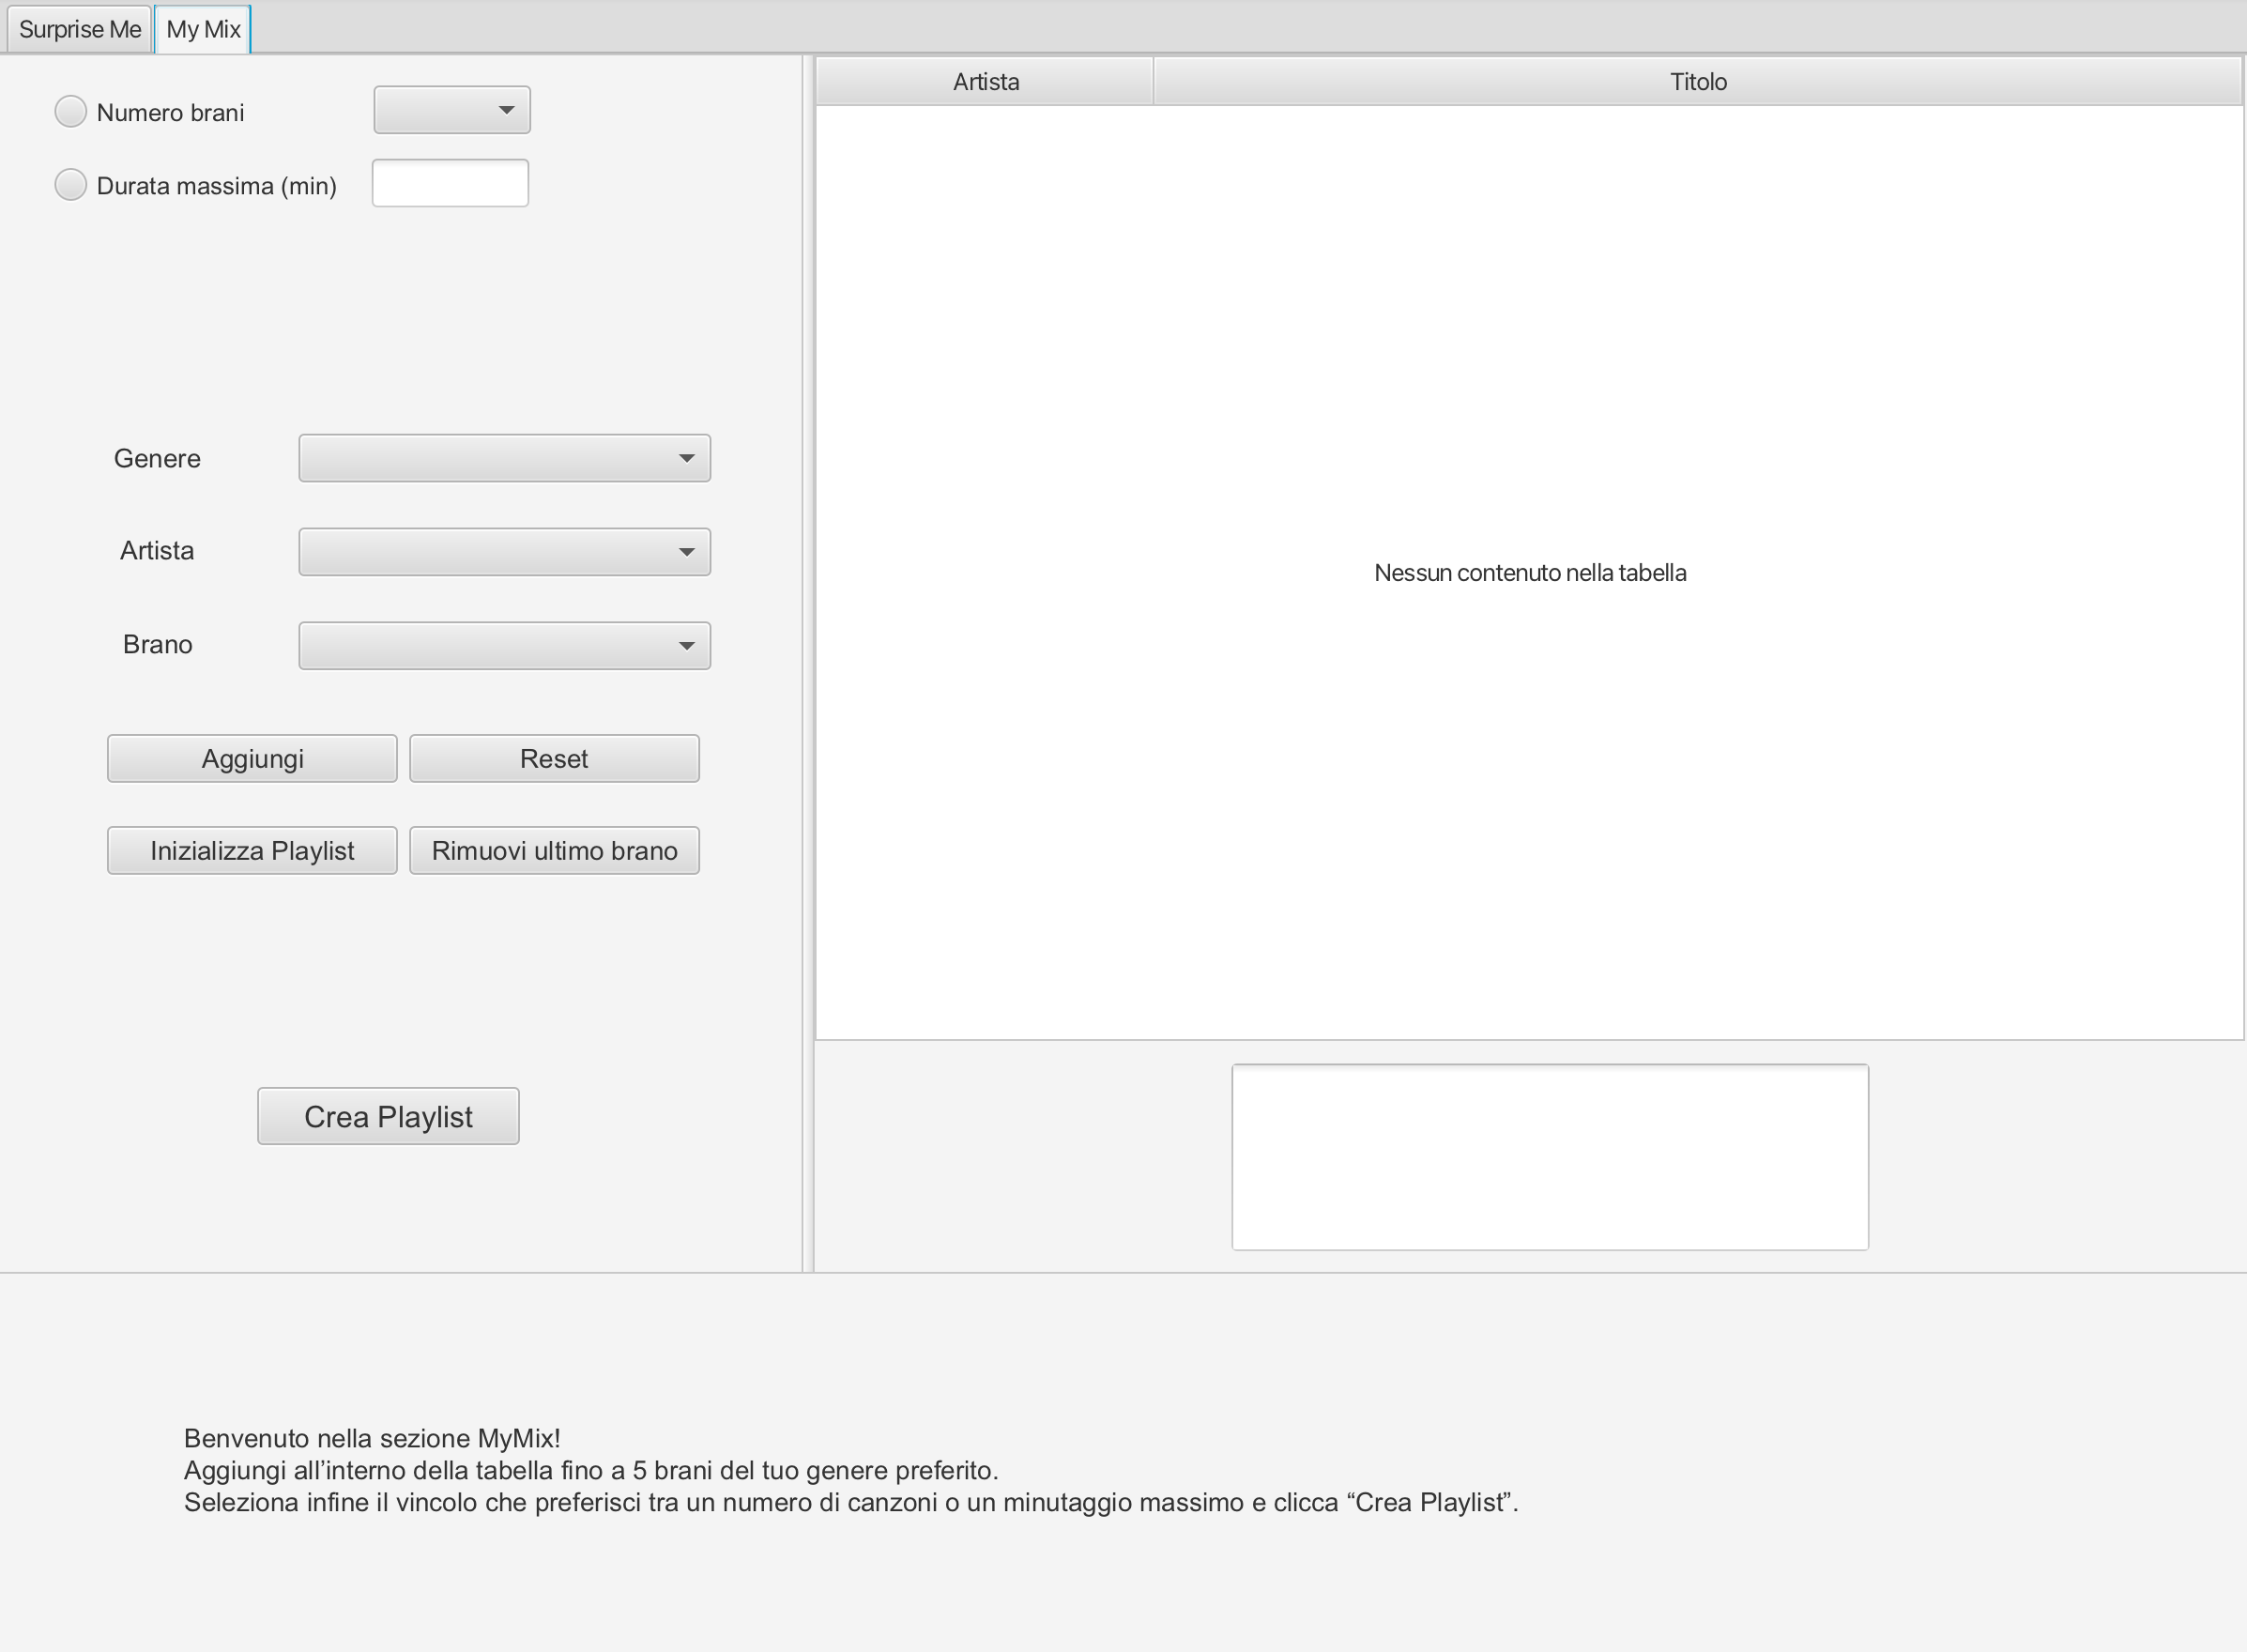
\includegraphics[clip, width=0.65\linewidth]{images/myMixTotal.png}
  \caption{My Mix tab}
\end{figure}


\newpage

\section{Strutture dati e algoritmi principali}

Nella realizzazione dell'applicazione, sono stati adottati sia il modello architetturale MVC (Model-View-Controller) che il design pattern DAO (Data Access Object). \\Queste metodologie permettono di separare chiaramente le principali componenti di un software, ovvero la logica, l'accesso ai dati e l'interfaccia utente. A seguire, verranno analizzati in dettaglio.

\subsection{Package it.polito.PlaylistGen}

\subsubsection{FXMLController}
Il Controller funge da mediatore tra la View e il Model, gestendo gli input utente, coordinando le azioni dell'applicazione e assicurandosi che l'interfaccia utente sia sincronizzata con lo stato interno dell'applicazione.
Di seguito sono riportati i metodi principali:

\begin{itemize}

\item \textbf{Acquisizione del vincolo scelto dall'utente}

Il vincolo scelto avviene prima apprendendo in quale sezione si trovi l'utente:

\begin{lstlisting}
// 0 = Surprise Me, 1 = My Mix
Integer nTab = tabPane.getSelectionModel().getSelectedIndex(); 
\end{lstlisting}

La definizione dei vincoli avviene attraverso le due variabili \textbf{isVincoloBrani} e \textbf{vincolo}. Il primo è \textit{True} se l'utente vuole una playlist con \textit{n} brani, \textit{False} se, invece, desidera che la lunghezza della playlist sia limitata dai minuti totali di ogni traccia.

È riportato come esempio l'acquisizione dei vincoli nel caso \textit{nTab = 0}.

\begin{lstlisting}
if (nTab == 0) {
			if (nBraniSurprise.isSelected()) {
				Integer vincolo = cmbNBraniSurprise.getValue();
				if (vincolo != null) {
					errorLabelSurprise.setText(null);
					this.setVincolo(vincolo);
					this.setIsVincoloBrani(true);
					return true;
				} else {
					errorLabelSurprise.setText("Inserire numero di brani massimo richiesto e riprovare");
					return false;
				}
			} else if (minBraniSurprise.isSelected()) {
				String input = choiceDurataMaxSurprise.getText();
				try {
					Integer vincolo = Integer.parseInt(input);
					if (vincolo > 180) {
						errorLabelSurprise.setText("Inserire valore inferiore a 180 minuti e riprovare");
						return false;
					} else {
						errorLabelSurprise.setText(null);
						this.setVincolo(vincolo);
						this.setIsVincoloBrani(false);
						return true;
					}
				} catch (Exception e) {
					errorLabelSurprise.setText("Inserire valore valido e riprovare");
					return false;
				}
			} else {
				else {
				
					...
					// Segnalazione errori all'utente
					...
					
				}
			}
		}
\end{lstlisting}

Il motivo per cui non si accetti un vincolo di minutaggio superiore a 180 minuti è puramente a fine prestazionale. Questa scelta sarà motivata nella sezione \textit{Risultati ottenuti}.

\item Acquisizione dei valori degli Slider (Sezione Surprise Me)
\begin{lstlisting}
	private void collectSliders() {

		Double energy = sliderEnergy.getValue();
		Double dance = sliderDance.getValue();
		Double valence = sliderValence.getValue();
		Double acoustic = sliderAcoustic.getValue();
		Double popularity = sliderPop.getValue();

		model.createPreference(energy, dance, valence, acoustic, popularity);
		
	}
\end{lstlisting}
\newpage
\item Acquisizione dei brani inseriti nella TableView (Sezione My Mix)
\begin{lstlisting}
@FXML
	void addTrackMix(ActionEvent event) {

		// Acquisisco valori scelti
		String genre = cmbGenreMix.getValue();
		String artist = cmbArtistMix.getValue();
		String title = cmbTrackMix.getValue();

		if (playlistTableMix.getItems().size() < 5) {
			if (title != null) {

				Track track = model.getTrackbyInput(genre, artist, title);
				if (track != null) {

					// Resetto ErrorLabel
					errorLabelMix.setText(null);

					// Aggiungo tracia a tabella MyMix e tabella di riferimento nel modello
					playlistTableMix.getItems().add(track);
					model.addTrackToMapId(track);

					// Blocco cambio del genere
					cmbGenreMix.setDisable(true);
					cmbGenreMix.setValue(genre);

					// Preparo prossima scelta
					this.resetChoiceMix(event);

				} else {
				
					...
					// Segnalazione errori all'utente
					...
					
				}
	}

\end{lstlisting}
Il primo controllo impedisce all'utente di inserire più di cinque brani all'interno della tabella, i restanti invece assicurano che l'utente non abbia lasciato nessuna Combobox a valore nullo. 

Una volta inserito il primo brano, l'unico limite è l'aggiunta di brani di genere diverso dall'appena selezionato.

\newpage
\item Avvio della ricerca Surprise Me
\begin{lstlisting}
@FXML
	void avviaRicercaSurprise(ActionEvent event) {
		
		if (this.findVincolo()) {
			this.disableVincoliSurprise();
			this.collectSliders();
			String genre = cmbGenreSurprise.getValue();
			String artist = cmbArtistSurprise.getValue();
			if (genre != null) {
				// Creo Grafo
				this.model.creaGrafoSurprise(genre, artist, model.getPreference());


				// Avvio ricerca
				List<Track> playlist = new ArrayList<>();
				playlist = model.calcolaPlaylist(artist, this.isVincoloBrani, this.vincolo, false);

				// Aggiungo output alla tabella
				this.playlistTableSurprise.getItems().clear();
				this.playlistTableSurprise.getItems().addAll(playlist);

				// Informazioni sulla playlist creata
				String durata = model.getDurataPlaylistSec(playlist);
				textAreaProgressSurprise
						.setText("Playlist Creata!\nNumero brani: " + playlist.size() + ".\nDurata totale: " + durata);

			} else {
				errorLabelSurprise.setText("Selezionare un genere e riprovare");
			}
		}

	}
\end{lstlisting}

Gli unici due controlli effettutati nel controller prima di avviare la ricerca sono l'inserimento di un vincolo tra i due disponibili e di un genere preferito su cui basare la creazione del grafo, poiché ogni vertice sarà un brano del genere scelto.

\newpage
\item Avvio della ricerca My Mix
\begin{lstlisting}
@FXML
	void avviaRicercaMix(ActionEvent event) {
		
		if (this.findVincolo()) {
			this.disableVincoliMix();
			if (!this.playlistTableMix.getItems().isEmpty()) {
				// Blocco opzione "Aggiungi" e "Reset"
				addTrack.setDisable(true);
				resetChoiceMix.setDisable(true);
				buttonremoveLastTrack.setDisable(true);

				// Creo Grafo
				model.creaGrafoMix(cmbGenreMix.getValue());

				// Avvio ricerca
				List<Track> playlist = new ArrayList<>();
				playlist = model.calcolaPlaylist(null, this.isVincoloBrani, this.vincolo, true);

				// Aggiungo output alla tabella
				this.playlistTableMix.getItems().clear();
				this.playlistTableMix.getItems().addAll(playlist);


				// Informazioni sulla playlist creata
				String durata = model.getDurataPlaylistSec(playlist);
				textAreaProgressMix
						.setText("Playlist Creata!\nNumero brani: " + playlist.size() + ".\nDurata totale: " + durata);

			} else {
				
					...
					// Segnalazione errori all'utente
					...
					
			}
		}

	}
\end{lstlisting}
Per la sezione "My Mix" invece il controllo sulla scelta del genere è sostituito dalla necessità che l'utente abbia scelto almeno un brano su cui calcolare i propri gusti musicali.
\end{itemize}

\newpage
\subsection{Package it.polito.PlaylistGen.db}


Questo pacchetto agevola l'interfacciamento con la base di dati seguendo il design pattern DAO. Comprende due classi:
\begin{itemize}
\item \texttt{DBConnect.java}, che contiene i parametri necessari per l'accesso al database e stabilisce la connessione con il medesimo.
\item \texttt{TracksDAO.java}, responsabile dell'estrazione dei dati dal database. Al suo interno, sono implementati tutti i metodi contenenti le query SQL utilizzate per interrogare la base di dati.
\end{itemize}

\subsubsection{DBConnect}

Il framework scelto per accedere database relazionale è HikaruCP\footnote{https://github.com/brettwooldridge/HikariCP}. Questo framework, sviluppato da Brett Wooldridge nel 2012, è basato sul concetto di connection pooling.

La connection pooling è un noto modello di accesso ai dati. Il suo scopo principale è ridurre il sovraccarico coinvolto nell'esecuzione delle connessioni al database e nelle operazioni di lettura/scrittura del database.

Le connessioni al database sono operazioni piuttosto costose e, pertanto, dovrebbero essere ridotte al minimo in ogni possibile caso d'uso (nei casi estremi, semplicemente evitate).

Il connection pooling implementa un contenitore di connessioni al database, che ci consente di riutilizzare un certo numero di connessioni esistenti, potendo così risparmiare efficacemente il costo di eseguire un grande numero di costose operazioni di accesso al database. Questo migliora le prestazioni complessive delle applicazioni basate su database.

Di seguito è riportato il codice per l'accesso al database:

\begin{lstlisting}
import java.sql.Connection;
import java.sql.SQLException;

import com.zaxxer.hikari.HikariConfig;
import com.zaxxer.hikari.HikariDataSource;

public class DBConnect {
		
	private static final String jdbcURL = "jdbc:mariadb://localhost/Spotify";
	public static HikariDataSource ds;
		
	public static Connection getConnection() {
			
		if (ds == null) {
			HikariConfig config = new HikariConfig();
			config.setJdbcUrl(jdbcURL);
			config.setUsername("user");
			config.setPassword("password");
				
			// configurazione MySQL
			config.addDataSourceProperty("cachePrepStmts", "true");
			config.addDataSourceProperty("prepStmtCacheSize", "250");
			config.addDataSourceProperty("prepStmtCacheSqlLimit", "2048");
				
			ds = new HikariDataSource(config);
		}
			
		try {	
			return ds.getConnection();
		} catch (SQLException e) {
			System.err.println("Errore connessione al DB");
			throw new RuntimeException(e);
		}
	}

}
\end{lstlisting}

L'username e la password per l'accesso al database SQL sono state sostituite per motivi di sicurezza.

\subsubsection{TracksDAO}

All'interno della classe \texttt{TracksDAO.java} troviamo i seguenti metodi per l'interrogazione del database, il metodo completo sarà riportato solo nell'ultimo esempio a scopo dimostrativo:
\begin{itemize}
\item Richiesta di tutti i generi presenti nel dataset
\begin{lstlisting}
public List<String> listAllGenre(){
		
		String sql = "SELECT Tracks.`Top Genre`, COUNT(Tracks.`Top Genre`) "
				+ "FROM Tracks "
				+ "GROUP BY Tracks.`Top Genre` "
				+ "HAVING COUNT(Tracks.`Top Genre`) >= 30";
		List<String> result = new ArrayList<String>();

		// ...
	}
\end{lstlisting}
\newpage
\item Richiesta di tutti gli artisti associati ad uno specifico genere
\begin{lstlisting}
public List<String> listAllArtistByGenre(String genre){
		
		String sql = "SELECT DISTINCT Tracks.`Artist`\n"
				+ "FROM Tracks\n"
				+ "WHERE Tracks.`Top Genre` = ? ";
		List<String> result = new ArrayList<String>();

		// ...
	}
\end{lstlisting}
\item Richiesta di tutti i brani associati ad uno specifico artista
\begin{lstlisting}
public List<String> listAllTracksByArtist(String artist){
		
		String sql = "SELECT DISTINCT Tracks.`Title`\n"
				+ "FROM Tracks\n"
				+ "WHERE Tracks.`Artist` = ? ";
		List<String> result = new ArrayList<String>();

		// ...
	}
\end{lstlisting}
\item Richiesta di tutti i brani associati ad uno specifico genere.
\begin{lstlisting}
public List<Track> listTracksByGenre(String genre) {
		
		String sql = "SELECT * \n"
				+ "FROM Tracks\n"
				+ "WHERE Tracks.`Top Genre`= ? ";
		List<Track> result = new ArrayList<Track>();

		// ...
		
	}
\end{lstlisting}
\newpage
\item Richiesta dei valori corrispondenti di un brano associato ad uno specifico genere, artista e titolo.
\begin{lstlisting}
public List<Track> listTracksByGenre(String genre) {
		
		String sql = "SELECT * \n"
				+ "FROM Tracks\n"
				+ "WHERE Tracks.`Top Genre`= ? ";
		List<Track> result = new ArrayList<Track>();

		try {
			Connection conn = DBConnect.getConnection();
			PreparedStatement st = conn.prepareStatement(sql);
			st.setString(1, genre);
			ResultSet res = st.executeQuery();
			
			while (res.next()) {

				Track track = new Track(res.getInt("Index"), res.getString("Title"), res.getString("Artist"), genre, res.getInt("Length (Duration)"), res.getInt("Year"),
						res.getInt("Energy"), res.getInt("Danceability"), res.getInt("Valence"), res.getInt("Acousticness"), res.getInt("Popularty"));

				
				result.add(track);
			}
			conn.close();
			return result;
			
		} catch (SQLException e) {
			e.printStackTrace();
			return null;
		}
		
	}

\end{lstlisting}
\end{itemize}

\newpage
\subsection{Package it.polito.PlaylistGen.model}

Nel pattern architetturale Model-View-Controller (MVC),
il "Model" rappresenta la componente responsabile della gestione dei dati e della logica dell'applicazione.\\Il ruolo principale del Model è separare la logica di presentazione (View) dalla logica di elaborazione (Model) e dal controllo delle interazioni dell'utente (Controller).

\subsubsection{Model}

Nella classe Model (\texttt{Model.java}), troviamo tutti i metodi di rilevanza algoritmica tra cui la ricorsione che verrà analizzata nel capitolo successivo.
Gli algoritmi principali sono i seguenti:
\begin{itemize}
\item Calcolo e aggiunta degli archi del grafo

Poiché ogni vertice del grafo è rappresentato dalla classe Vertex, il vero problema computazionale è stato aggiungere gli archi che avessero un peso al di sotto di una soglia prestabilita, al fine di non creare un grafo completo e rendere la ricerca scarsa dal punto di vista prestazionale.
Come soglia massima di peso è stato scelta la media del peso degli archi del grafo completo precedentemente creato (funzione \texttt{trovaAvg()}), al fine di eliminare circa metà degli archi e assicurarsi comunque una soluzione finale soddisfacente.
\begin{lstlisting}
	private void creaArchi() {

		// Creo Archi
		for (Vertex vi : this.grafo.vertexSet()) {
			for (Vertex vj : this.grafo.vertexSet()) {
				Integer viTrackId = vi.getTrack().getTrackId();
				Integer vjTrackId = vj.getTrack().getTrackId();
				if (viTrackId != vjTrackId) {
					Double weight = Math.abs(vi.getScore() - vj.getScore());
					Graphs.addEdgeWithVertices(this.grafo, vi, vj, weight);
				}
			}
		}
		// Al fine di ottimizzare la ricerca, elimino ogni arco di peso inferiore alla media degli archi
		Integer avg = this.trovaAvg();
		for (Vertex vi : this.grafo.vertexSet()) {
			for (Vertex vj : this.grafo.vertexSet()) {
				if (this.grafo.getEdge(vi, vj) != null) {
					if (this.grafo.getEdgeWeight(this.grafo.getEdge(vi, vj)) < avg) {
						this.grafo.removeEdge(vi, vj);
					}
				}
			}
		}
	}
\end{lstlisting}
\newpage
\item Calcolo dei gusti musicali usando i brani in input (Sezione "My Mix")

\begin{lstlisting}
private Preference calcolaPreferenze() {

	// Energy
	Double sumEnergy = 0.0;
	// Danceability
	Double sumDanceability = 0.0;
	// Valence
	Double sumValence = 0.0;
	// Acoustic
	Double sumAcoustic = 0.0;
	// Popularity
	Double sumPopularity = 0.0;

	for (Track ti : this.tracksInput.values()) {
		sumEnergy += ti.getEnergy();
		sumDanceability += ti.getDanceability();
		sumValence += ti.getValence();
		sumAcoustic += ti.getAcousticness();
		sumPopularity += ti.getPopularty();
	}

	Double avgEnergy = sumEnergy / this.tracksInput.size();
	Double avgDanceability = sumDanceability / this.tracksInput.size();
	Double avgValence = sumValence / this.tracksInput.size();
	Double avgAcoustic = sumAcoustic / this.tracksInput.size();
	Double avgPopularity = sumPopularity / this.tracksInput.size();

	// Divido ciascun fattore per 10 per rendere i punteggi consistenti con quelli della prima sezione (da 1 a 10)
	Double finalEnergy = (double) Math.round(avgEnergy / 10);
	Double finalDanceability = (double) Math.round(avgDanceability / 10);
	Double finalValence = (double) Math.round(avgValence / 10);
	Double finalAcoustic = (double) Math.round(avgAcoustic / 10);
	Double finalPopularity = (double) Math.round(avgPopularity / 10);

	preference = new Preference(finalEnergy, finalDanceability, finalValence, finalAcoustic, finalPopularity);
	return preference;
	}
\end{lstlisting}
\newpage
\end{itemize}

\subsubsection{Preference}

La classe Preference (\texttt{Preference.java}) offre la possibilità di conservare le informazioni relative ai gusti dell'utente.

\begin{lstlisting}
public class Preference {
	
	private Double energy;
	private Double danceability;
	private Double valence;
	private Double acousticness;
	private Double popularty;
	
	public Preference(Double energy, Double danceability, Double valence, Double acousticness, Double popularty) {
		super();
		this.energy = energy;
		// ...
		this.popularty = popularty;
	}
\end{lstlisting}

\subsubsection{Track}

La classe Track (\texttt{Track.java}) è responsabile per definire le istanze delle canzoni e permette di memorizzare all'interno del programma i dati estratti dal dataset.

\begin{lstlisting}
public class Track {

	private Integer trackId;
	private String title;
	private String artist;
	private String genre;
	private Integer length;
	private Integer year;
	private Integer energy;
	private Integer danceability;
	private Integer valence;
	private Integer acousticness;
	private Integer popularty;
	
	public Track(Integer trackId, String title, String artist, String genre, Integer length, Integer year, Integer energy, Integer danceability, Integer valence, Integer acousticness, Integer popularty) {
		super();
		this.trackId = trackId;
		// ...
		this.popularty = popularty;
	}
\end{lstlisting}

\subsubsection{Vertex}

La classe Vertex (\texttt{Vertex.java}), invece, racchiude le due informazioni sopracitate in un'unica classe, rappresentando il singolo vertice del grafo su cui verrà effettuata la ricorsione.

\begin{lstlisting}
public class Vertex {

	private Track track;
	private Double score;

	public Vertex(Track track, Double score) {
		super();
		this.track = track;
		this.score = score;
	}

\end{lstlisting}

\newpage
\section{Ricorsione}

L'approccio per l'ottenimento della playlist ottima si basa su una ricerca esaustiva (backtracking) per esplorare tutte le possibili combinazioni di brani e costruire la playlist migliore rispettando i vincoli dati. Questo tipo di approccio, pur potendo risultare dispendioso in termini di memoria e complessità temporale, è giustificato dal vincolo di un massimo di 40 brani totali (circa 2 ore e 30 minuti). L'inserimento di questo vincolo permette di ottenere un risultato in tempi sotto il secondo e confida nel fatto che difficilmente un utente possa ascoltare musica per più del tempo sopracitato senza cambiare manualmente brano o genere.

Il metodo principale \texttt{CalcolaPlaylist} inizia inizializzando e resettando le variabili di stato dell'algoritmo, ottiene la lista di brani validi (\texttt{canzoniValide}) e una lista parziale di brani (\texttt{parziale}) inizializzata in base alle preferenze dell'utente (Mix o SurpriseMe) ed effettua infine la chiamata al metodo ricorsivo \texttt{calcola} per trovare la migliore playlist possibile.

\begin{lstlisting}
public List<Track> calcolaPlaylist(String artist, Boolean isVincoloBrani, Integer vincolo, Boolean isMix) {

		this.resetSearch();

		List<Vertex> canzoniValide = new ArrayList<Vertex>();
		ConnectivityInspector<Vertex, DefaultWeightedEdge> ci = new ConnectivityInspector<>(this.grafo);
		List<Vertex> parziale = new ArrayList<>();

		// Controllo se i vincoli richiesti sono raggiungibili dal grafo
		if (isVincoloBrani && this.getNVertici() < vincolo) {
			vincolo = this.getNVertici();
		} else if (!isVincoloBrani && this.getTotalDurataGraph() < vincolo) {
			vincolo = this.getTotalDurataGraph();
		}

		// Sezione Mix, aggiungo vertici corrispondenti ai brani inseriti alla soluzione parziale
		if (isMix) {
			for (Track ti : this.tracksInput.values()) {
				for (Vertex vi : this.getVertici(artist, preference)) {
					if (ti.equals(vi.getTrack())) {
						parziale.add(vi);
					}
				}
			}
			// Comincio ricerca a partire dall'ultimo brano inserito
			canzoniValide.addAll(ci.connectedSetOf(parziale.get(parziale.size() - 1)));

		} else { // Sezione SurpriseMe, aggiungo miglior inizio possibile
			Vertex start = findBestStart(artist);
			parziale.add(start);

			// Trovo componente connessa di "start"
			canzoniValide.addAll(ci.connectedSetOf(start));

		}

		calcola(parziale, canzoniValide, isVincoloBrani, vincolo);

		for (Vertex vi : this.bestPlaylist) {
			this.finalPlaylist.add(vi.getTrack());
		}
		return this.finalPlaylist;
\end{lstlisting}

Il metodo ricorsivo \texttt{calcola} prende come input una lista \texttt{parziale} che rappresenta una possibile playlist parziale, una lista di \texttt{canzoniValide} che sono i brani disponibili per essere aggiunti alla playlist, un flag \texttt{isVincoloBrani} che indica se esiste un vincolo sul numero di brani o sulla durata totale della playlist, e un parametro \texttt{vincolo} che rappresenta il valore massimo del vincolo.
Il metodo segue i seguenti step:
\begin{enumerate}
\item Itera attraverso la lista di \texttt{canzoniValide} e cerca di aggiungere ciascun brano (\texttt{Vertex vi}) alla playlist parziale, rispettando eventuali vincoli imposti.
\item Aggiorna ricorsivamente la playlist e calcola la somma degli archi pesati di questa playlist parziale.
\item Se la somma degli archi è inferiore al miglior punteggio (\texttt{bestScore}), continua la ricorsione. Altrimenti, verifica se la playlist parziale attuale è migliore di quella salvata come migliore fino a quel momento (\texttt{bestPlaylist}). Se è così, aggiorna la migliore playlist e il miglior punteggio.

\begin{lstlisting}
	private void calcola(List<Vertex> parziale, List<Vertex> canzoniValide, Boolean isVincoloBrani, Integer vincolo) {

		for (Vertex vi : canzoniValide) {
			if (!parziale.contains(vi)) {
				if (!this.isVincoloSuperato(vi, parziale, isVincoloBrani, vincolo)) {
					parziale.add(vi);
					Double sommaArchiProvvisoria = this.getSommaArchi(parziale);
					if (sommaArchiProvvisoria < bestScore) {
						this.calcola(parziale, canzoniValide, isVincoloBrani, vincolo);
					}
					parziale.remove(parziale.size() - 1);
				} else {
					// Controllo soluzione migliore La soluzione migliore corrisponde al cammino con somma dei pesi degli archi piu' bassa
					Double sommaArchiProvvisoria = this.getSommaArchi(parziale);
					if (sommaArchiProvvisoria < bestScore) {
						this.bestPlaylist = new ArrayList<>(parziale);
						this.bestScore = sommaArchiProvvisoria;
					}
				}
			}
		}

	}
\end{lstlisting}
\end{enumerate}

\newpage
\section{Diagramma delle classi}

\begin{figure}[h]
  \centering
  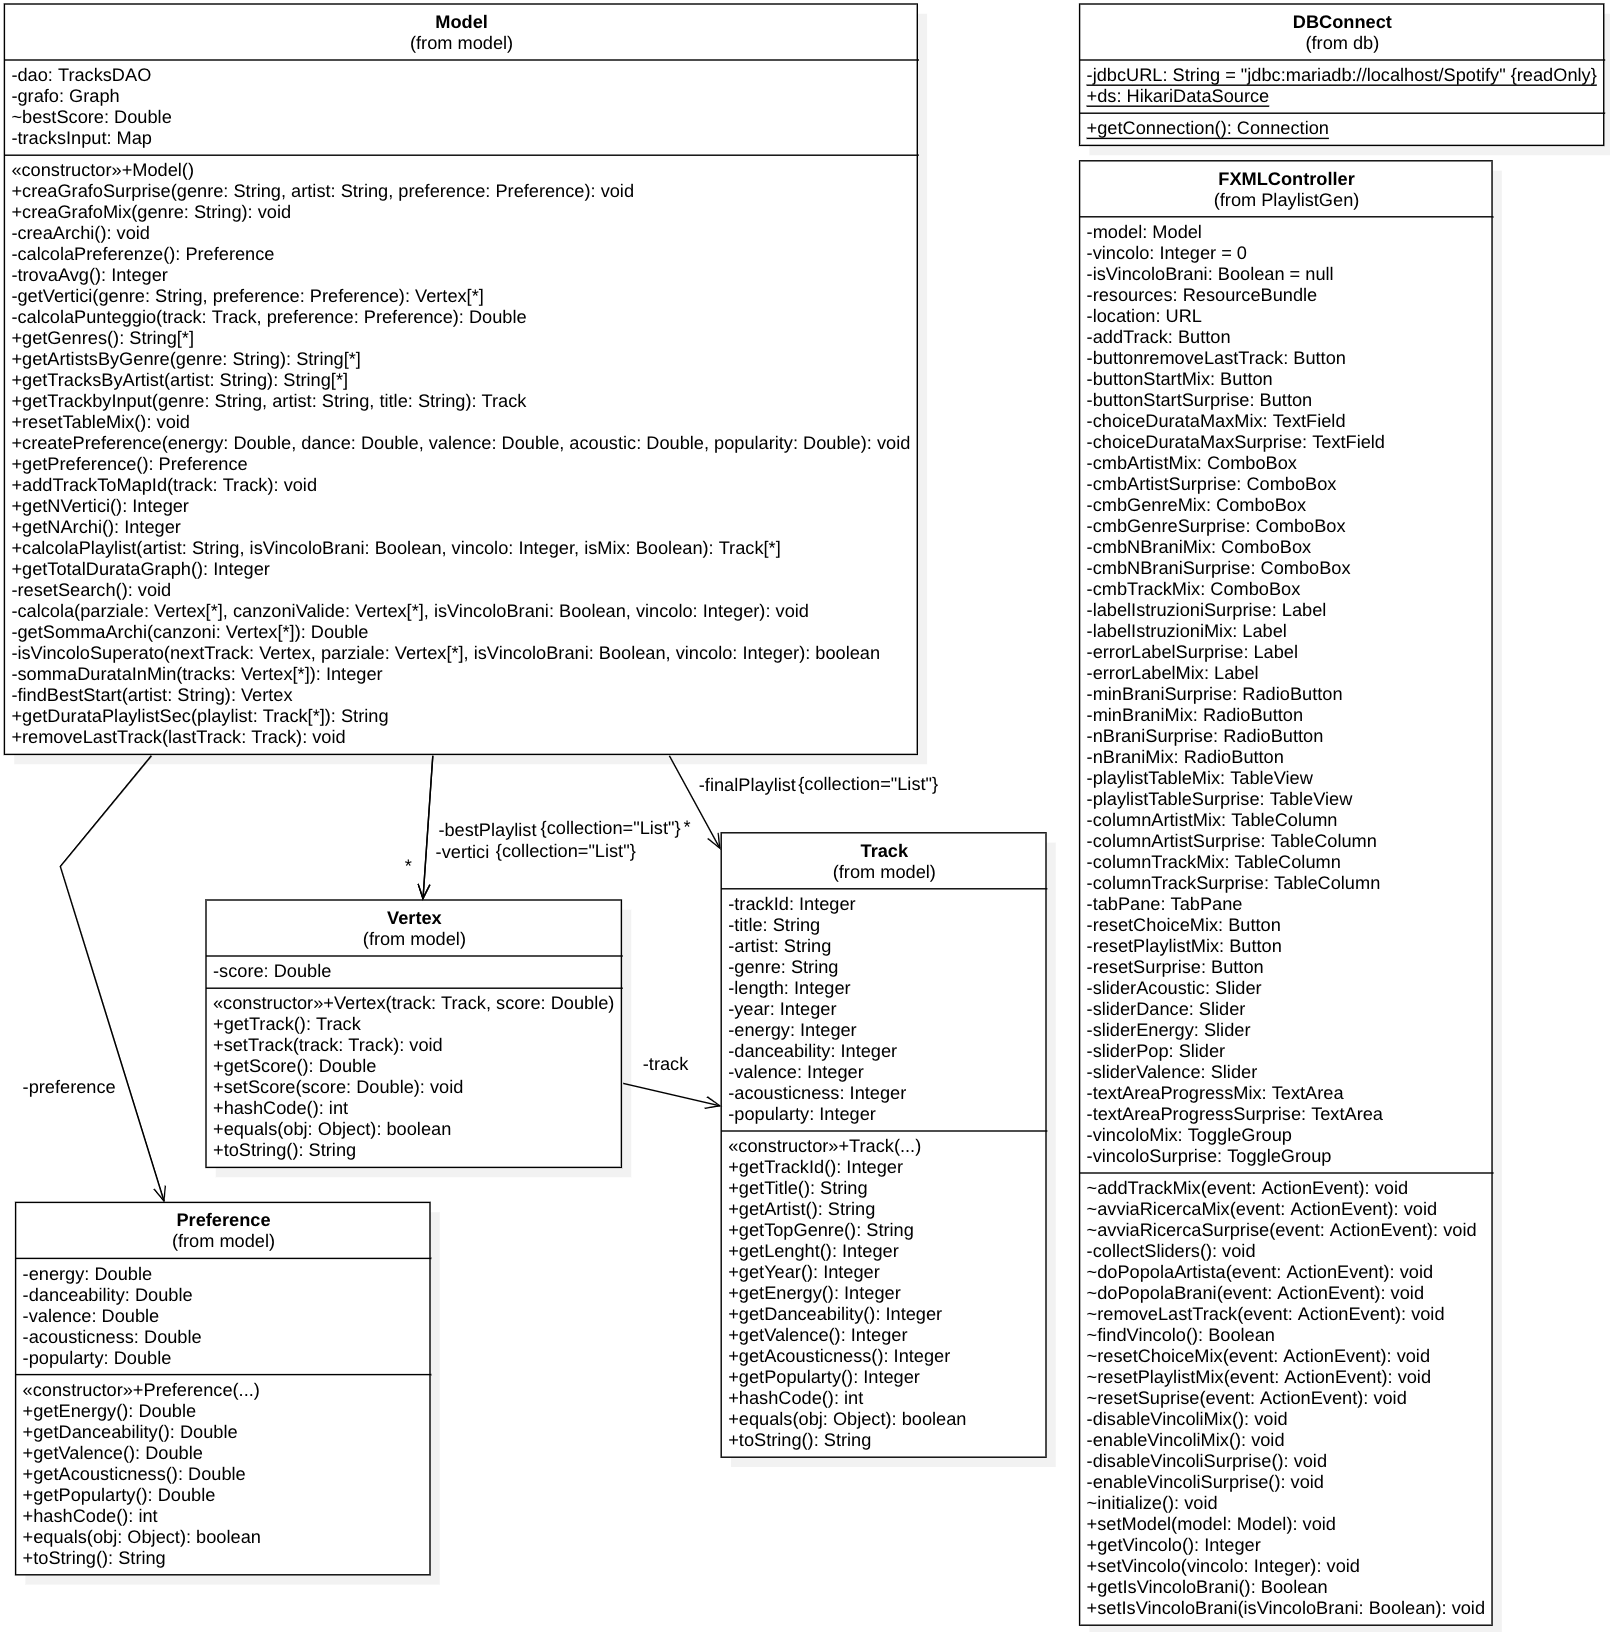
\includegraphics[scale=0.50]{images/diagram}
\end{figure}

\newpage
\section{Risultati ottenuti e considerazioni finali}

Il prodotto finale risulta particolarmente performante anche lavorando con generi contenenti numerosi brani, permettendo di produrre il risultato in tempistiche sempre al di sotto del secondo fino a un massimo vincolo di 40 canzoni (in media poco meno di tre ore di minuti totali).

Nella figura sottostante è possibile notare l'andamento delle performance all'aumentare del numero di canzoni richiesto nella playlist della Tab Surprise Me. In questo esempio, a fine puramente esemplificativo, gli Slider Energia (E), Ballabilità (D), Positività (V), Acustica (A) e Popolarità (P) sono stati posizionati rispettivamente a 2, 4, 6, 8 e 10. \par  
I generi presi in considerazione nell'esempio sono i tre maggiormente popolati di brani, al fine di visionare l'andamento nella peggiore delle situazioni computazionali. I generi in questione sono Rock (164 brani), Pop (156 brani) ed European Pop (150 brani).

\begin{figure}[h]
\centering
  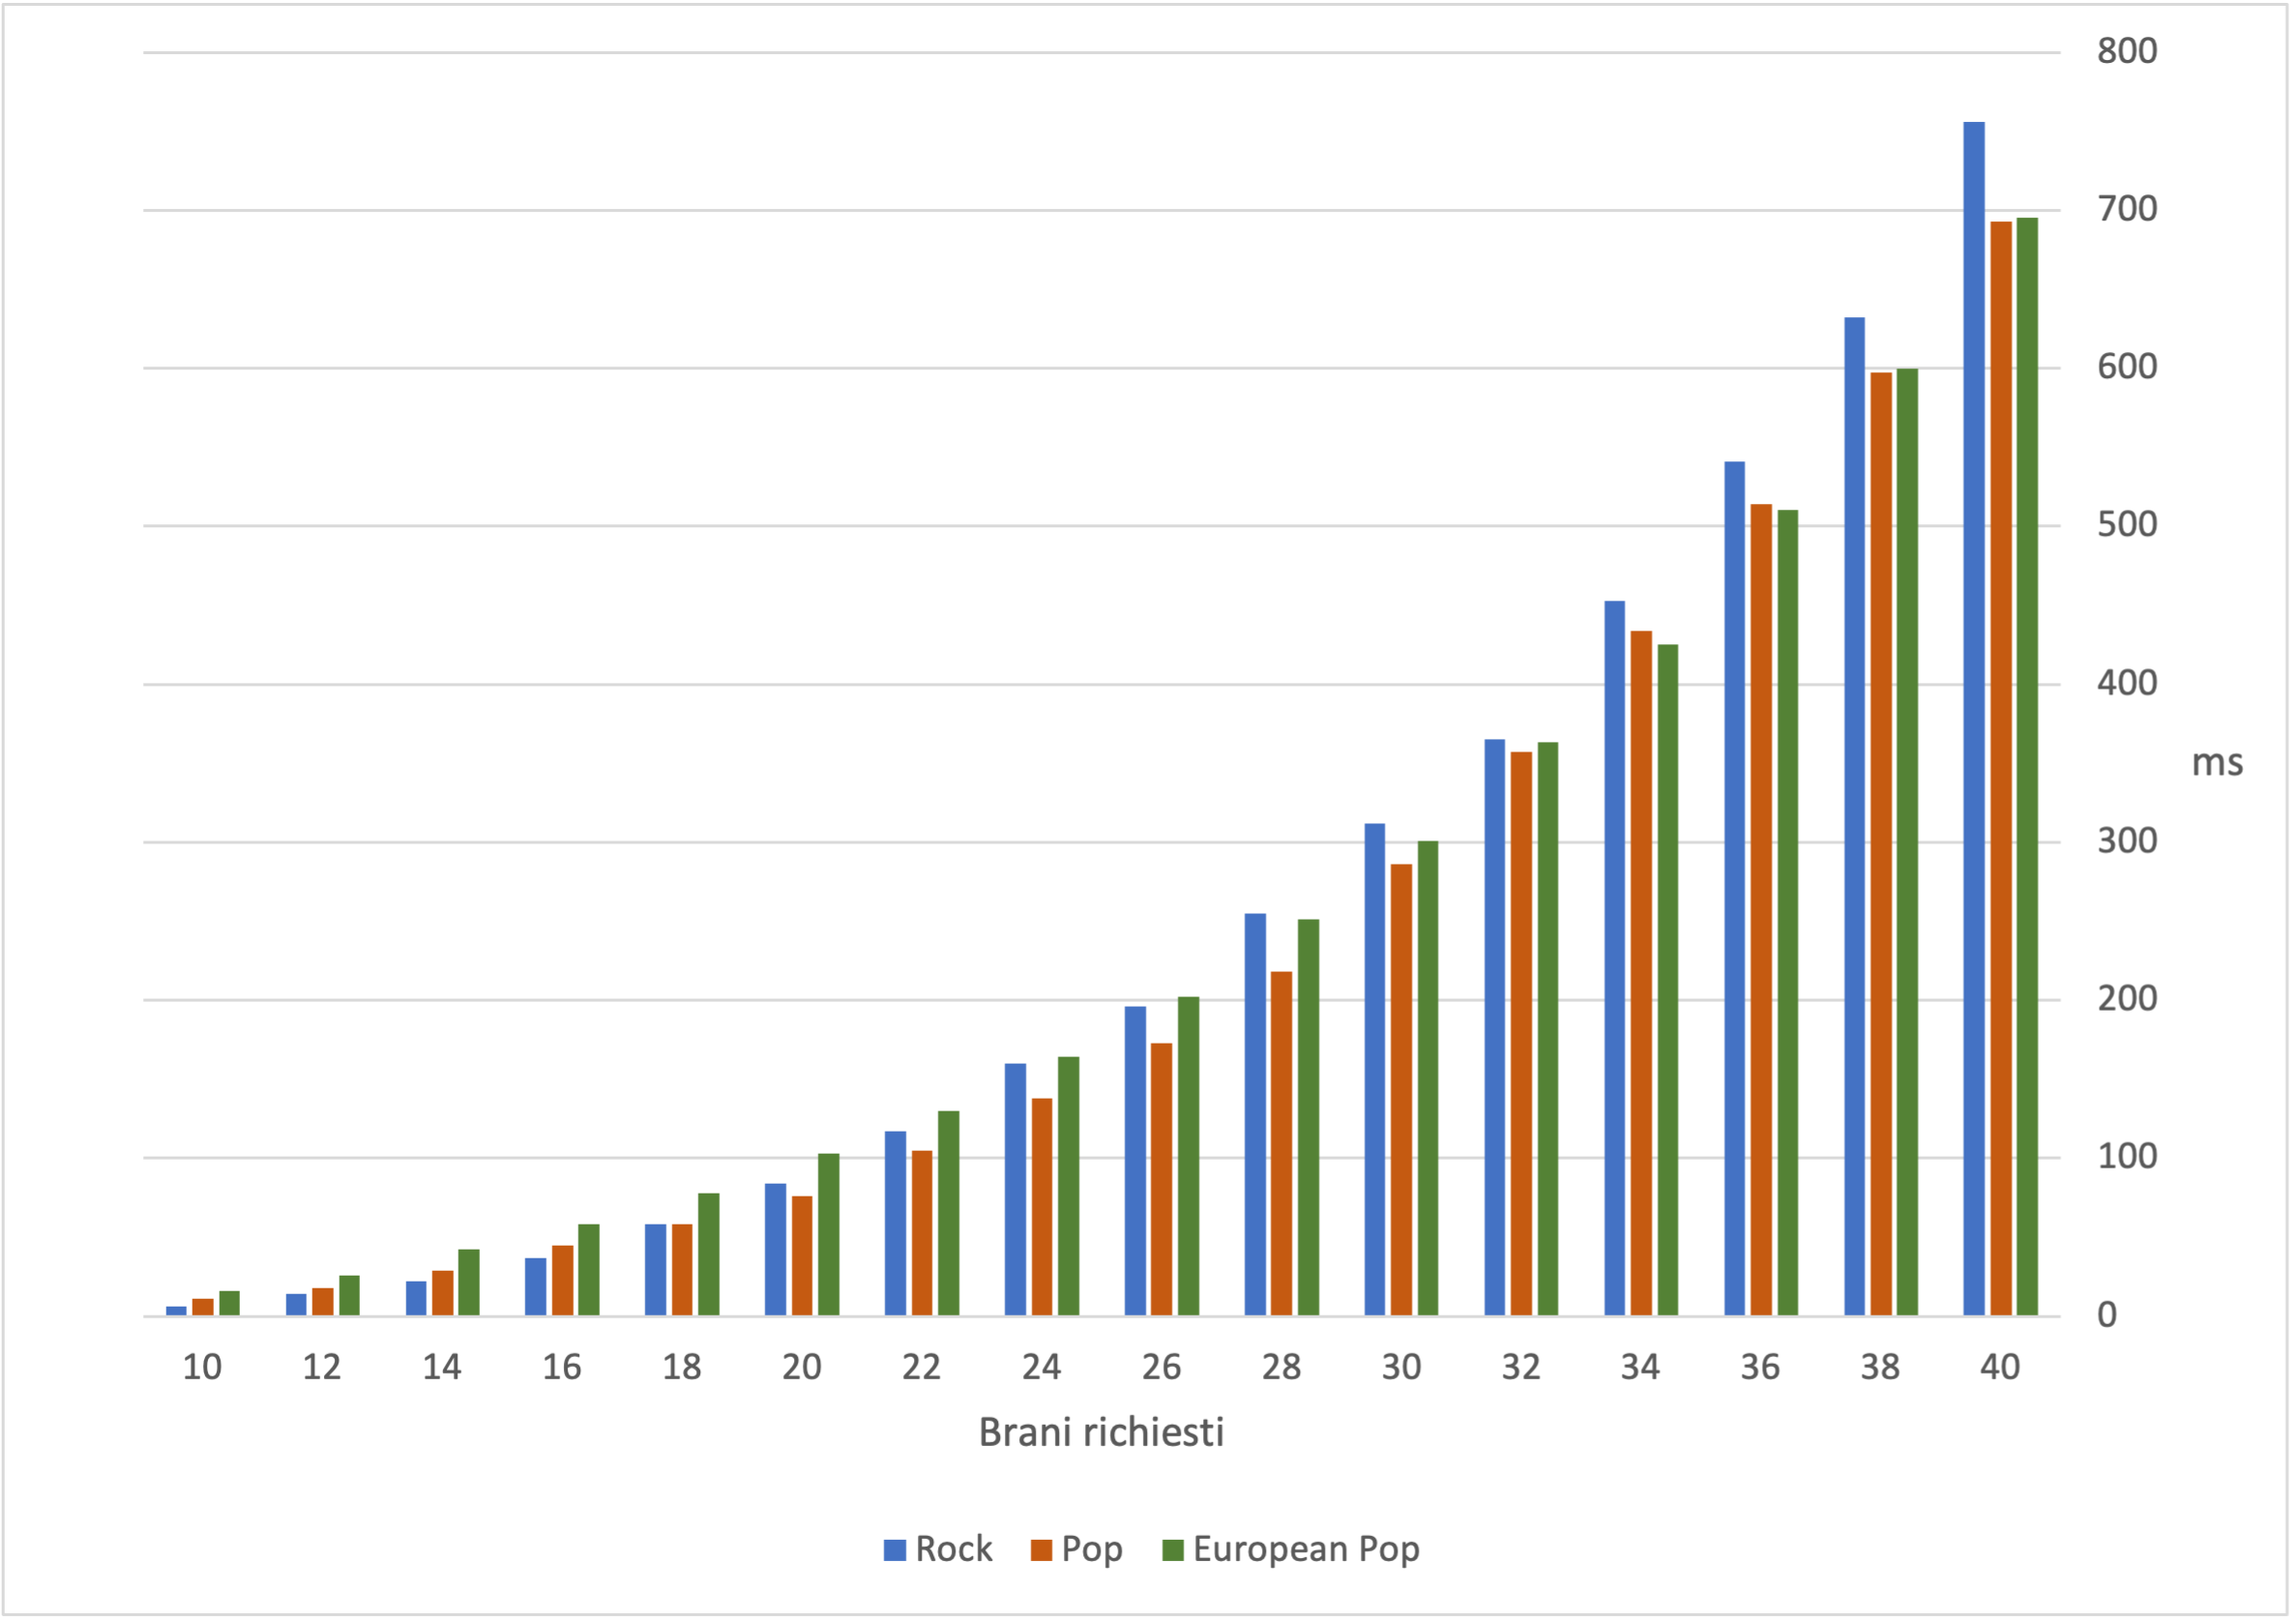
\includegraphics[scale=0.50]{images/performance}
  \label{performance}
  \caption{Tempo di completamento all'aumentare del numero di brani richiesti}
\end{figure}

È possibile ora concludere indicando quali siano le criticità di questo progetto e possibili implementazioni future:
\begin{itemize}
\item Scalabilità: andando ad aumentare il volume di dati musicali, l'algoritmo deve essere in grado di gestire la crescita senza perdere in efficienza, cosa che non può essere garantita con il tipo di ricorsione esaustiva implementato. Nel futuro sarebbe il caso di sostituirlo con un algoritmo più pratico e accettabile in grado di trovare soluzioni approssimate ma che richiedono meno risorse.
\item Valutazione oggettiva della playlist: definire metriche oggettive per valutare la qualità di una playlist può essere complicato. L'algoritmo dovrebbe cercare di fornire un risultato che sia gradevole ed apprezzato dagli utenti.
\item Requisiti dell'utente e gusti musicali variabili: gli utenti hanno gusti musicali molto variabili e soggettivi. Un algoritmo potrebbe avere difficoltà a soddisfare le preferenze individuali di ciascun utente, specialmente se sono mutevoli nel tempo. Una possibilità futura potrebbe essere quella di implementare nuovi vincoli più specifici e meglio rappresentativi della richiesta dell'utente.
\end{itemize}
\newpage

Il progetto completo è disponibile al seguente indirizzo: 

https://github.com/TdP-prove-finali/MarraCarlo

Al seguente link è disponibile una video dimostrazione del progetto:

https://youtu.be/eR-s5fUmcfQ



\newpage
\section*{Licenza d'uso}
\begin{center}
 Sviluppo di un'applicazione software per la generazione automatica di playlist attraverso la ricerca ricorsiva e grafi pesati  © 2023\\ by Carlo Marra\\ is licensed under CC BY-NC-SA 4.0
\end{center}

\end{document}